% !TEX program = pdflatex
% !BIB program = biber

%% One can optionally have all this inside a separate setup.tex
% !TEX program = pdflatex
% !BIB program = biber

% !TEX root = main.tex
\documentclass[10pt, a4paper]{article}
% \documentclass[12pt, a4paper, oneside]{memoir}
% \chapterstyle{veelo}

%% Sets page size and margins
\usepackage[a4paper,top=3cm,bottom=2cm,left=3cm,right=3cm,marginparwidth=1.75cm]{geometry}
%\usepackage[left=2cm,top=2cm,bottom=2cm,bindingoffset=1cm]{geometry}

\usepackage[utf8x]{inputenc}
\usepackage{graphicx}
\usepackage{float}
\usepackage{imakeidx}
\usepackage{amsmath}
\usepackage[colorlinks=true, allcolors=blue]{hyperref}
\usepackage{graphicx}
\usepackage{float}
\usepackage{imakeidx}
\usepackage{amsmath}
\usepackage{url}
\usepackage[export]{adjustbox}
\usepackage{subcaption}
\usepackage{booktabs}
\usepackage{pdflscape}
\usepackage[table,xcdraw]{xcolor}
%\usepackage{svg}

%% Useful packages
\usepackage[colorinlistoftodos]{todonotes}
\usepackage[T1]{fontenc}

%% Language and font encodings
\usepackage[english]{babel}

%% Define a few colours to be used throughout the document
\usepackage{tikz,xcolor}
\definecolor{TextColor}{HTML}{000000}
\definecolor{SideColorDark}{HTML}{000000}
\definecolor{MainColor}{HTML}{0000FF}
\definecolor{OppositeColor}{HTML}{FF0000}
\definecolor{HighlightColor}{HTML}{FFFF00}


%% Code block style
%  Load the \ttfamily font
\usepackage[T1]{fontenc}
\usepackage[scaled]{beramono}

%  Format code blocks
\usepackage{listings}
%  Change caption name
\renewcommand*{\lstlistingname}{Code block}
\captionsetup[lstlisting]{margin=0cm,format=hang,font=small,format=plain,labelfont={bf,up},textfont={it}}
%  Style
\lstset{
  showstringspaces=false,
  formfeed=\newpage,
  commentstyle=\itshape,
  backgroundcolor=\color{gray!5},
  breakatwhitespace=false,         % sets if automatic breaks should only happen at whitespace
  breaklines=true,                 % sets automatic line breaking
  captionpos=b,                    % sets the caption-position to bottom
  commentstyle=\color{gray},    % comment style
  escapeinside={\%*}{*)},          % if you want to add LaTeX within your code
  keepspaces=true,
  numbersep=2mm,                   % how far the line-numbers are from the code
  showspaces=false,
  showstringspaces=false,
  showtabs=false,
  stepnumber=1, numberfirstline=false,
  basicstyle=\linespread{1}\footnotesize\ttfamily,
  keywordstyle=\bfseries\color{MainColor},
  stringstyle=\itshape\color{OppositeColor},
  numberstyle=\footnotesize\ttfamily\color{gray},
  numbers=left,xleftmargin=4mm,framexleftmargin=0mm,xrightmargin=0mm,
  frame=top,frame=bottom,
}

\title{Insert title here}
\author{Daniel Robinson\\18361137}

\begin{document}
% \maketitle
    \begin{titlepage}
        \begin{center}
            \vspace*{1cm}
            
            \begin{figure}
			\centering
            
\includegraphics[scale=2]{UScrest-top.jpg}
            \end{figure}
            
            \huge
            \textbf{Project Management\\Assignment 1}
            
            \vspace{1.5cm}
            
            \large
            Peter\\
            12345678\\
            \vspace{0.5cm}
            Biance\\
            12345678\\
            \vspace{0.5cm}
            Carmen\\
            12345678\\
            \vspace{0.5cm}
            Eduard\\
            12345678\\
            \vspace{0.5cm}
            Sarel\\
            12345678\\
            \vspace{0.5cm}
            Daniel Robinson\\
            18361137\\
            \vspace{3.5cm}
            
            \large
            Date: 7 February 2017
            
        \end{center}
\end{titlepage}

\newpage

% \begin{abstract}
% Your abstract.
% \end{abstract}


\section*{Plagiarism Declaration}

I know that plagiarism is wrong.\\\\
\noindent
Plagiarism is to use another's work (even if it is summarised, translated or rephrased) and pretend that it is one's own. This assignment is our own work.\\\\
\noindent
Each contribution to and quotation (e.g. "cut and paste") in this assignment from the work(s) of other people has been explicitly attributed, and has been cited and referenced. In addition to being explicitly attributed, all quotations are enclosed in inverted commas, and long quotations are additionally in indented paragraphs.\\\\
\noindent
I have not allowed, and will not allow, anyone to use my work (in paper, graphics, electronic, verbal or any other format) with the intention of passing it off as his/her own work.\\\\
\noindent
I know that a mark of zero may be awarded to assignments with plagiarism and also that no opportunity be given to submit an improved assignment.\\\\
\noindent
I know that students involved in plagiarism will be reported to the Registrar and/or the Central Disciplinary Committee.

\section*{Executive Summary}
In today's day and age, engineers are expected to be versatile in more aspects than ever before. One of these is project management. This assignment hopes to introduce and ready engineering students for project management and as close to reality as possible. For example, the teams of students are multi-disciplinary, and had most probably not had prior experience working together.\\

\noindent
For this particular assignment, a project structure / 'blueprint' has been designed in order to manage the creation of a beer brewery.

\newpage
\tableofcontents
\listoffigures
\listoftables

\newpage
\section{Introduction}

\section{Project Scope Statement}
\subsection{Objectives}

A local micro-brewery will be designed and constructed in the Stellenbosch area. The main objective of this product/service is to design a local brewery for in the Stellenbosch area, that will have a deliverance of 3 600 000 draft beers per annum which is equivalent to 1 800 000 liters.\\

\noindent
Other objectives include the following:
\begin{itemize}
\item Designing a brewery that will be able to cater as a bar that can be used by the public of Stellenbosch.
\item To create a product that is economically viable for the target market namely students.
\item To create a local product that will make use of local based – products.
\item To create a building that is environmentally friendly and also aesthetically appealing.
\end{itemize}

\subsubsection{Project Objectives}

The objective of this project is to efficiently utilize the resources, manage the time and cost of the project.\\

\noindent
The project must be completed within the budget of \$380 000.\\

\noindent
The project must be completed within the 9 month period which will start

\subsection{Deliverables}

To ensure that the project stays on track the deliverables are submitted to approve the continuation of the project. These intermediate checks are listed below.

\begin{itemize}
\item \emph{Market Assessment}\\
Conducting a market research study with information about possible customers, prefaces and needs.
\item \emph{Business evaluation}\\
Set up a preliminary budget and cost of the project. Identify the target market
\item \emph{Design \& development}\\
Designing necessary plans and schematizations of the project. Identify the specifications and technical requirements needed for the project.
\item \emph{Market}\\
Setting up of Responsibility allocations and timetable for the marketing program.
\item \emph{Risk Analysis}\\
Identify the possible risks that will influence the project negatively and have an effect on the timeline and budget of the project.
\item \emph{Develop Design}\\
Set up a finalized design with all engineering specifications and that are in alignment with the customers requirements.
\item \emph{Identify possible Vendors \& set up RFQ}\\
Set up a requests for quotes developed and issued.
\item \emph{Prototype Development}\\
Develop a functional prototype that is based on the final product design This prototype is then evaluated.
\item \emph{Process Engineering Plan}\\
Set up a supply chain network for a larger scale production.
\item \emph{Production plan}\\
Manufacturing, engineering and quality control signed approval. Machinery implemented for production. Set up schedule for delivering based on sales forecast.
\item \emph{Assess or RFQ}\\
Review RFQ’s and specify the terms of the contract.
\item \emph{Product Launch}\\
Product is officially signed off from manufactures and launched into the industry.
\item \emph{Production Pilot Test}\\
Run a test of the production with normal operation and staff. Assess whether any errors occur or if changes need to be made.
\end{itemize}

\subsection{Milestones}

\begin{landscape}

\begin{table}[!h]
\centering
\caption{Milestones}
\label{tab:milestones}
\begin{tabular}{lllll}
Milestone & Critical Path Tasks                   & Task Group          & Task Duration (Days) & Target Date \\\hline
1         & Evaluate Market                       & Market Assessment   & 12                   & 27-04-2017  \\
          & Develop Business Opportunity          &                     & 14                   &             \\
          & Customer Preference Study             &                     & 21                   &             \\
          & Business Evaluation (NPV, etc.)       &                     & 4                    &             \\\hline
2         & Design and Development Plan           & Design              & 6                    & 06-06-2017  \\
          & Design Specifications                 &                     & 22                   &             \\\hline
3         & Advertising Campaign                  & Commercialization   & 28                   & 14-07-2017  \\\hline
4         & Design Labeling                       & Design              & 5                    & 03-08-2017  \\
          & Approve Design                        &                     & 4                    &             \\
          & Initial Engineering Specifications    & Engineering         & 5                    &             \\\hline
5         & Design Verification Activities        & Engineering         & 7                    & 01-09-2017  \\
          & Verification Design Review            &                     & 4                    &             \\
          & Release Pre-production Specifications &                     & 10                   &             \\\hline
6         & Build Functional Model                & Engineering         & 18                   & 27-09-2017  \\\hline
7         & Issue Sample (Production Equivalent)  & Procurement         & 5                    & 24-10-2017  \\
          & Perform Supplier Process Capability   & Supplier Quality    & 14                   &             \\\hline
8         & Process Engineering Plan              & Manufacturing       & 15                   & 14-11-2017  \\\hline
9         & Validation Design Review              & Engineering         & 4                    & 24-11-2017  \\
          & Approve Model Design                  &                     & 4                    &             \\\hline
10        & Qualify Supplier                      & Supplier Quality    & 10                   & 08-12-2017  \\
          & Design Transfer Activities            & Engineering         & 7                    &             \\
          & Product Release Meetings              & Engineering Quality & 3                    &             \\\hline
11        & Develop Production Control Plan       & Manufacturing       & 8,5                  & 08-01-2018  \\
          & Approve Production Parts              &                     & 5                    &             \\
          & Contracting for Deliveries            &                     & 8                    &             \\\hline
12        & Submit Production Purchase Order      & Manufacturing       & 2                    & 31-01-2018  \\
          & Production Pilot Test                 &                     & 5                    &             \\
          & Debugging Production System           &                     & 4                    &             \\
          & Production Release                    &                     & 3                    &             \\
          & Product Launch                        & Commercialization   & 3                    &             \\
\end{tabular}
\end{table}

\end{landscape}

\begin{landscape}

\subsection{Work Breakdown Structure}

\begin{figure}[H]
\centering
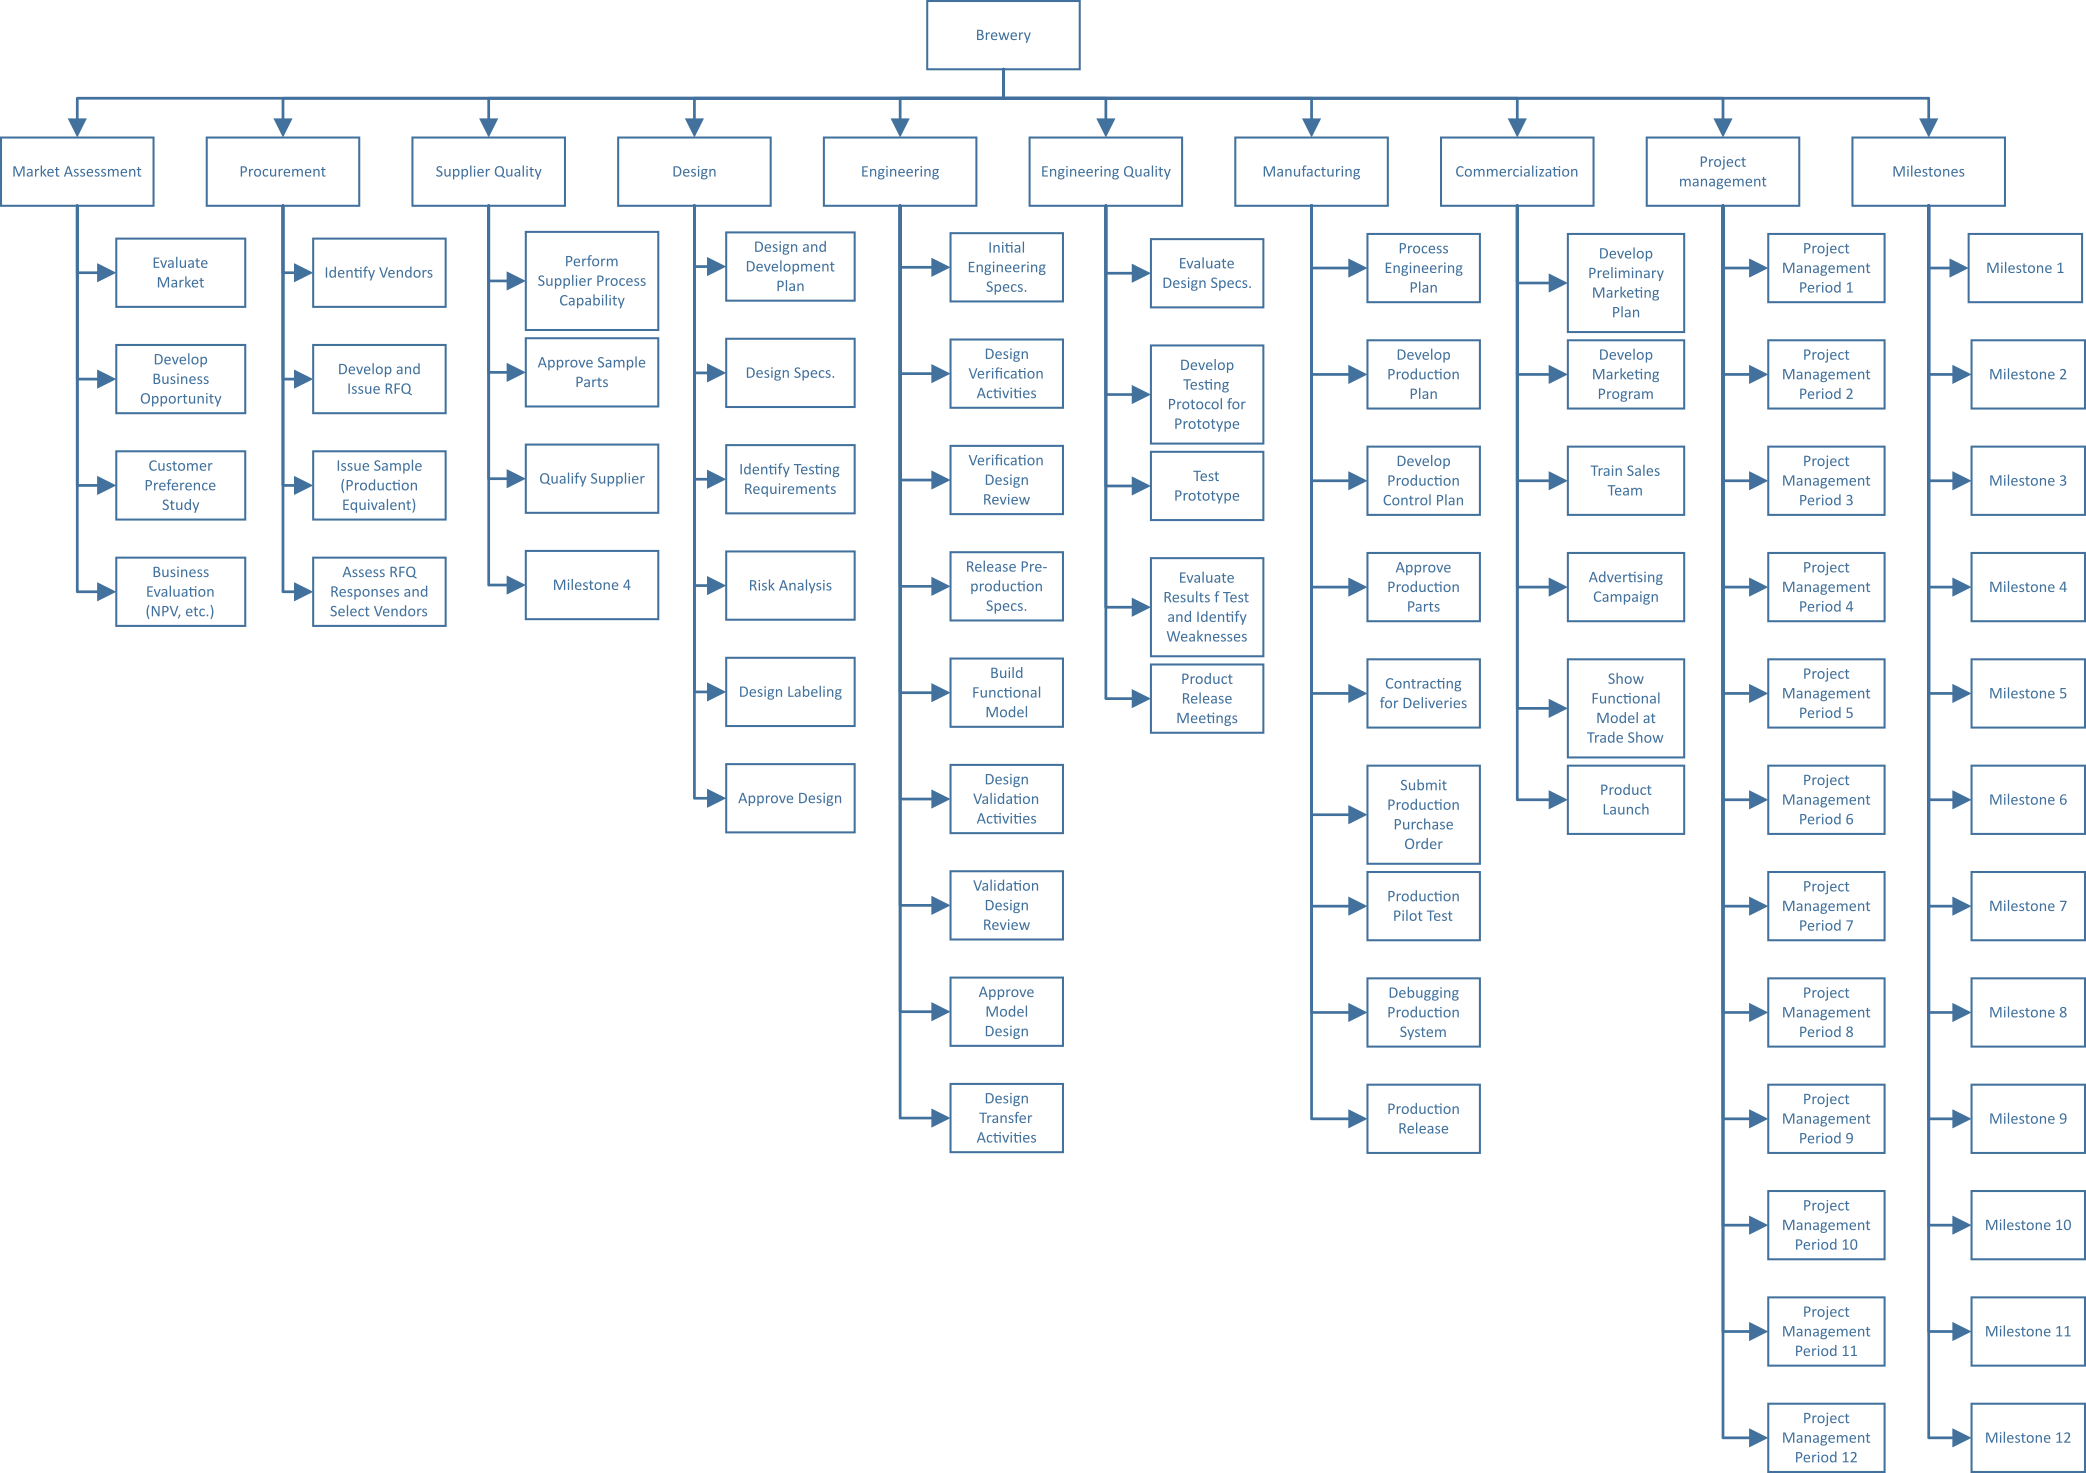
\includegraphics[scale=0.85]{WBS.png}
%\includesvg[scale=0.65,angle=90,origin=c]{WBS}
%\caption{Work Breakdown Structure}
\label{fig:wbs}
\end{figure}

\end{landscape}

\subsection{Technical Requirements}
\subsubsection{Summary of product}

There are four types of beer that need to be manufactured namely: Weiss, Ale and two different flavoured lagers. All the beers utilize the same brewing system with slight alterations needed to create each unique beer. These alterations include different fermenting processes and different grains used. There needs to be four brewing systems working simultaneously in order to produce a sufficient amount of all beers.

\subsubsection{Product Requirements}

\begin{itemize}
\item There should be 4 varieties of beer
\item Each beer will be sold in 500ml glasses
\item The temperature of the beer should always be carefully monitored from the brewing process until the product is sold to the customer 
\item Control systems should be put in place in order to monitor and control each stage of the brewing process 
\item The quality of the final product needs to be of a high standard in order to compete in the respective market 
\item The  final product should be marked at a reasonable price in order to appeal to a wider target market (students)
\item The process compromises of 12 stages that need to be carefully executed in order to produce the best possible product 
\end{itemize}
\subsubsection{Project Requirements}

\begin{itemize}
\item Project commences 20th February 2017 and terminates 3rd May 2017
\item All the suppliers of the company should be identified and have their capabilities assessed 
\item The final product must be designed completely. The components should include specifications, risk analysis, design analysis, production process and possible testing requirements.
\item A full quality assessment must be done throughout all stages of production of the final product
\end{itemize}

\subsection{Limits and Exclusions}
\subsubsection{Limits}
\subsubsection{Exclusions}
\subsection{Review and Approval} 

When developing a product or service for a client it is very important to keep client satisfaction in mind. If the client is not happy then there the feasibility of the project in general is compromised. If the project is not feasible there is market for the product or service because the customers will not buy it. This is why it is very important to do a feasibility study early on in the process. The feasibility study must ensure that the customer will be willing to spend money on this product or service. To determine if the product will be feasible the customer must evaluate the following; cost, the benefits of the project, the likelihood that the project will succeed and the reputation of the contractor that is used for the project.\\

\noindent
To be able to do a feasibility study all of the phases in the process need to be documented. These documents need to contain diagrams and schematic representations of the entire process and all the steps and resources that were used. By documenting everything it is easier for the customer to review all of the decisions made. It can also make it easier to see why these decisions were made. By making it easier for the customer to review the projects progress the contractor can be ensured of customer satisfaction. Customer approval procedure must be done regularly throughout the process, this ensures that if there are any errors early on in the process, they can be evaluated and alternative solutions can be made. By doing this regularly the contractor can ensure that the client stays satisfied throughout the process. If these errors are picked up early it can save the contractor a lot of money later in the process.

\section{Project Baseline Plan}
\subsection{Baseline Commentary}

\section{Project Budget}

The estimated budget and estimated hours provided by Sim4 project was used as a guideline of what should be spent during each period to ensure that the project would stay within the budget of \$380 000.\\

\noindent
To calculate the budget the effectiveness of the resources were brought into consideration. An assumption was made that all resources will work at an 80\% effectiveness rate. The estimated hours of each task as well as the safety margin of 80\% effectiveness was used to determine the hours worked for each task using the formula provided.\\

\begin{center}
$ Actual\ time\ worked\ (hours)\ =\ \frac{Estimated\ time\ (hours)}{\% effectiveness} $
\end{center}

The budget forecast is provided in Appendix \ref{appendix:budget}.

\subsection{Direct Resource Costs}

Table \ref{tab:resourcecosts} provides the estimated cost of the different resources that will be hired. More than one engineer will be hired since the engineer will be working as a Project Manager for the period.

\begin{table}[]
\centering
\caption{Resource costs per hour}
\label{tab:resourcecosts}
\begin{tabular}{ll}
\textbf{Resources}          & \textbf{Rate} \\\hline
Engineer 1                  & \$58.00       \\
Engineer 2                  & \$42.00       \\
Junior Marketing Specialist & \$57.00       \\
Junior Product designer     & \$47.00       \\
Marketing Manager           & \$95.00       \\
Operation Specialist        & \$53.00       \\
Quality Engineer            & \$71.00       \\
Senior product designer     & \$84.00       \\
Engineer 3                  & \$55.00      
\end{tabular}
\end{table}

\subsection{Training and Events prospective costs}

There was decided that during the first period the engineer will be sent for training on project Management. This is to ensure that the engineer will be more effective as a project Manager. There was also decided to hire resources that are cheaper but have less skills and send them for training to improve their skills and effectiveness.\\

\noindent
Managerial actions will also be rewarded to resources to improve their work ethic and effictiveness.\\

\noindent
Table \ref{tab:actions} provides information regarding the different training and managerial actions that will take place during the provided timeline.

% Please add the following required packages to your document preamble:
% \usepackage[table,xcdraw]{xcolor}
% If you use beamer only pass "xcolor=table" option, i.e. \documentclass[xcolor=table]{beamer}
\begin{table}[]
\centering
\caption{Training and Managerial Actions costs}
\label{tab:actions}
\begin{tabular}{llllll}
\textbf{Period} & \textbf{Action}              & \textbf{Amount of People} & \textbf{Cost} & \textbf{Total Cost}                 &  \\
1               & Project Management           & 1                         & \$1,000.00    & \$1,000.00                          &  \\
                & Project Evaluation           & 1                         & \$1,000.00    & \$1,000.00                          &  \\
3               & Interpersonal training       & 2                         & \$600.00      & \$1,200.00                          &  \\
5               & company sponsored event      & 3                         & \$100.00      & \$300.00                            &  \\
6               & Pizza Party                  & 6                         & \$10.00       & \$60.00                             &  \\
                & Process Engineering          & 1                         & \$600.00      & \$600.00                            &  \\
8               & Management Recognition event & 4                         & \$50.00       & \$200.00                            &  \\
9               & Pizza Party                  & 6                         & \$10.00       & \$60.00                             &  \\
                & Negotiation techniques       & 2                         & \$600.00      & \$1,200.00                          &  \\
10              & Principles of Quality        & 1                         & \$600.00      & \$600.00                            &  \\
                & Pizza Party                  & 8                         & \$10.00       & \$80.00                             &  \\
11              & Milestone celebration        & 4                         & \$1,000.00    & \$4,000.00                          &  \\
                &                              &                           &               & \cellcolor[HTML]{FFFE65}\$10,300.00 & 
\end{tabular}
\end{table}

\subsection{Total Costs}

The total cost estimate of each period is listed Table \ref{tab:totalcosts}.

% Please add the following required packages to your document preamble:
% \usepackage[table,xcdraw]{xcolor}
% If you use beamer only pass "xcolor=table" option, i.e. \documentclass[xcolor=table]{beamer}
\begin{table}[]
\centering
\caption{Total estimated costs}
\label{tab:totalcosts}
\begin{tabular}{llllll}
\textbf{Period} & \textbf{Cost of period} & \textbf{Total cumulative cost} & \textbf{Budget Left over}           &  &  \\
Period 1        & \$57,920.00             & \$57,920.00                    & \$322,080.00                        &  &  \\
Period 2        & \$43,560.00             & \$101,480.00                   & \$278,520.00                        &  &  \\
Period 3        & \$60,420.00             & \$161,900.00                   & \$218,100.00                        &  &  \\
Period 4        & \$15,535.00             & \$177,435.00                   & \$202,565.00                        &  &  \\
Period 5        & \$19,185.00             & \$196,620.00                   & \$183,380.00                        &  &  \\
Period 6        & \$30,561.25             & \$227,181.25                   & \$152,818.75                        &  &  \\
Period 7        & \$18,865.00             & \$246,046.25                   & \$133,953.75                        &  &  \\
Period 8        & \$17,420.00             & \$263,466.25                   & \$116,533.75                        &  &  \\
Period 9        & \$10,850.00             & \$274,316.25                   & \$105,683.75                        &  &  \\
Period 10       & \$16,990.00             & \$291,306.25                   & \$88,693.75                         &  &  \\
Period 11       & \$27,452.50             & \$318,758.75                   & \$61,241.25                         &  &  \\
Period 12       & \$14,660.00             & \$333,418.75                   & \cellcolor[HTML]{9AFF99}\$46,581.25 &  &  \\
                &                         &                                &                                     &  & 
\end{tabular}
\end{table}

\section{Risk Assessment Plan}
\subsection{Risk identification}
\subsection{Risk Classification}

\newpage
%\section*{Appendices}
\begin{appendices}
%\subsection*{Appendix A: Budget Documentation and Analysis}
\section{Budget Documentation and Analysis}
\label{appendix:budget}

\subsection{Simulated Task Estimations}

\begin{figure}[H]
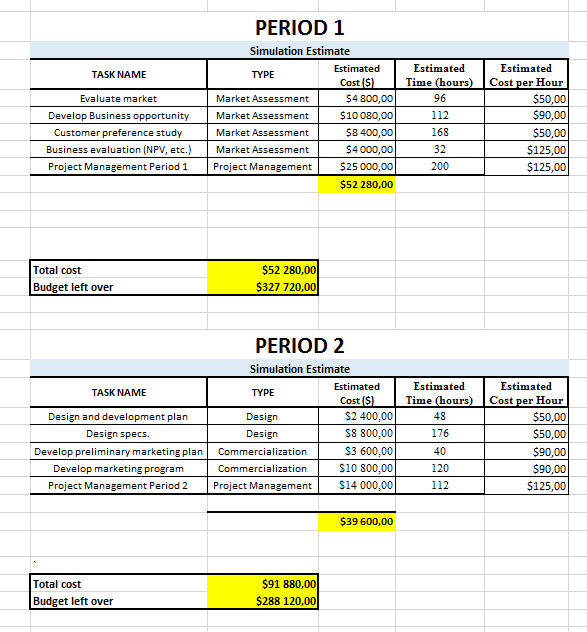
\includegraphics[scale=1]{budget_forecast_sim_12.PNG}
\caption{Budget Forecast from simulation (period 1 and 2)}
\end{figure}
\begin{figure}[H]
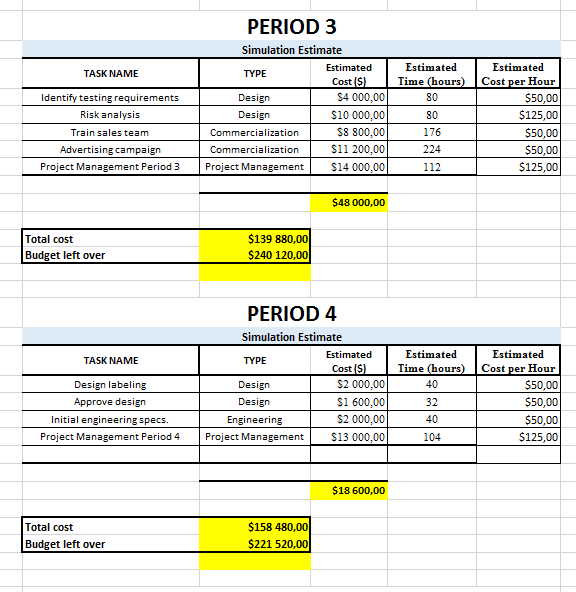
\includegraphics[scale=1]{budget_forecast_sim_34.PNG}
\caption{Budget Forecast from simulation (period 3 and 4)}
\end{figure}
\begin{figure}[H]
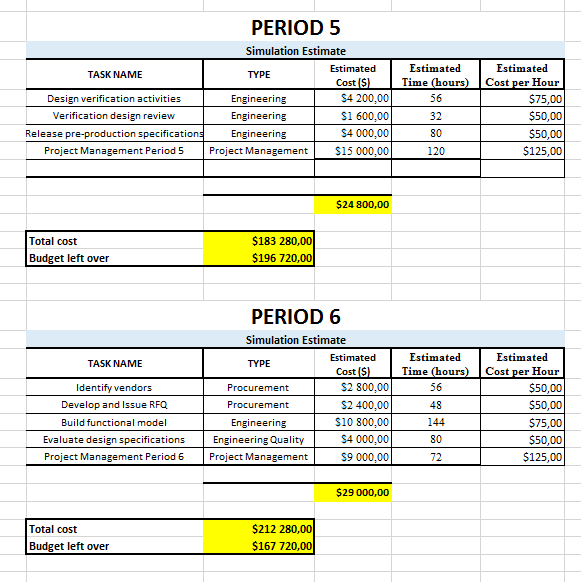
\includegraphics[scale=1]{budget_forecast_sim_56.PNG}
\caption{Budget Forecast from simulation (period 5 and 6)}
\end{figure}
\begin{figure}[H]
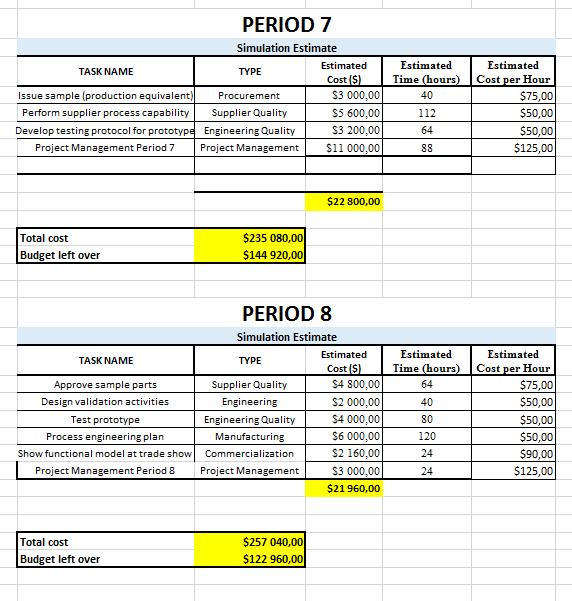
\includegraphics[scale=1]{budget_forecast_sim_78.PNG}
\caption{Budget Forecast from simulation (period 7 and 8)}
\end{figure}
\begin{figure}[H]
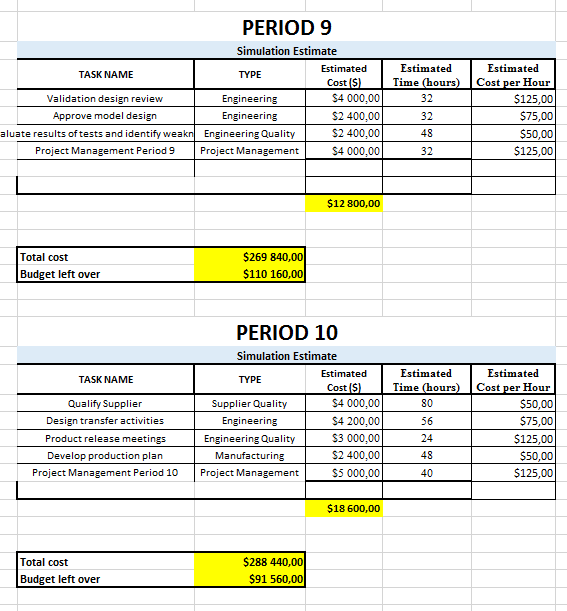
\includegraphics[scale=1]{budget_forecast_sim_910.PNG}
\caption{Budget Forecast from simulation (period 9 and 10)}
\end{figure}
\begin{figure}[H]
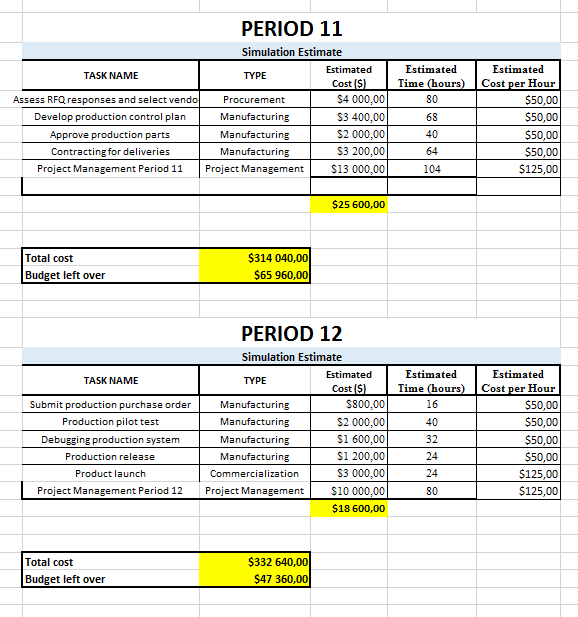
\includegraphics[scale=1]{budget_forecast_sim_1112.PNG}
\caption{Budget Forecast from simulation (period 11 and 12)}
\end{figure}


%\begin{landscape}

% Please add the following required packages to your document preamble:
% \usepackage[table,xcdraw]{xcolor}
% If you use beamer only pass "xcolor=table" option, i.e. \documentclass[xcolor=table]{beamer}
%\begin{table}[]
%\centering
%\caption{Budget forecast}
%\label{my-label}
%\begin{tabular}{lllllllllllllllllllllllll}
%\hline
%PERIOD 1 &  &  &  &  &  &  &  &  &  &  &  &  &  &  &  &  &  &  &  &  &  &  &  &  \\ \hline
%Simulation Estimate &  &  &  &  &  & Estimated Budget &  &  &  &  &  &  &  &  &  &  &  &  &  &  &  &  &  &  \\
%TASK NAME & TYPE & Est Cost (\$) & Est Time[h] & Est Cost/h &  &  & RESOURCES &  &  &  &  &  &  &  &  &  &  &  &  &  & MANAGERIAL Actions &  &  &  \\
%Evaluate market & Market Assessment & \$4 800,00 & 96 & \$50,00 &  & Devision & Estimated Hours & Assigned 1 &  &  &  &  &  & Assigned 2 &  &  &  &  &  & Total cost & Action & People & Cost & Total Cost \\
%Develop Business opportunity & Market Assessment & \$10 080,00 & 112 & \$90,00 &  &  &  & Resource name & Hours worked & \% effictive & Actual Hours & Rate & Cost & Resource name & Hours worked & \% effictive & Actual Hours & Rate & Cost &  &  &  &  &  \\
%Customer preference study & Market Assessment & \$8 400,00 & 168 & \$50,00 &  & Project Management & 200 & Engineer 1 & 200 & 90 & 222,2222222 & \$58,00 & \$12 888,89 &  &  &  &  &  &  & \$12 888,89 & Project Management & 1 & \$1 000,00 & \$1 000,00 \\
%Business evaluation (NPV, etc.) & Market Assessment & \$4 000,00 & 32 & \$125,00 &  & Market Assesment & 100 & Marketing Manager & 100 & 100 & 100 & \$95,00 & \$9 500,00 & Junior Marketing Specialist & 100 & 100 & 100 & \$57,00 & \$5 700,00 & \$15 200,00 & Project Evaluation & 1 & \$1 000,00 & \$1 000,00 \\
%Project Management Period 1 & Project Management & \$25 000,00 & 200 & \$125,00 &  & Market Assesment & 112 & Marketing Manager & 112 & 80 & 140 & \$95,00 & \$13 300,00 &  &  &  &  &  &  & \$13 300,00 &  &  &  &  \\
% &  & \cellcolor[HTML]{F8FF00}\$52 280,00 &  &  &  & Market Assesment & 32 & Junior Marketing Specialist & 32 & 80 & 40 & \$57,00 & \$2 280,00 &  &  &  &  &  &  & \$2 280,00 &  &  &  &  \\
% &  &  &  &  &  & Market Assesment & 96 & Junior Marketing Specialist & 96 & 80 & 120 & \$57,00 & \$6 840,00 &  &  &  &  &  &  & \$6 840,00 &  &  &  &  \\
% &  &  &  &  &  &  &  &  &  &  &  &  &  &  &  &  &  &  &  & \$50 508,89 &  &  &  & \$2 000,00 \\
% &  &  &  &  &  &  &  &  &  &  &  &  &  &  &  &  &  &  &  &  &  &  &  &  \\
%Total cost & \cellcolor[HTML]{F8FF00}\$52 280,00 &  &  &  &  & Total cost & \$52 508,89 &  &  &  &  &  &  &  &  &  &  &  &  &  &  &  &  &  \\
%Budget left over & \cellcolor[HTML]{F8FF00}\$327 720,00 &  &  &  &  & Budget left over & \$327 491,11 &  &  &  &  &  &  &  &  &  &  &  &  &  &  &  &  &  \\
% &  &  &  &  &  &  &  &  &  &  &  &  &  &  &  &  &  &  &  &  &  &  &  &  \\
% &  &  &  &  &  &  &  &  &  &  &  &  &  &  &  &  &  &  &  &  &  &  &  &  \\
% &  &  &  &  &  &  &  &  &  &  &  &  &  &  &  &  &  &  &  &  &  &  &  &  \\
% &  &  &  &  &  &  &  &  &  &  &  &  &  &  &  &  &  &  &  &  &  &  &  &  \\
% &  &  &  &  &  &  &  &  &  &  &  &  &  &  &  &  &  &  &  &  &  &  &  &  \\
% &  &  &  &  &  &  &  &  &  &  &  &  &  &  &  &  &  &  &  &  &  &  &  &  \\ \hline
%\end{tabular}
%\end{table}

% Please add the following required packages to your document preamble:
% \usepackage{booktabs}
%\begin{table}[]
%\centering
%\caption{Budget Forecast}
%\label{tab:budgetforecast}
%\begin{tabular}{@{}lllllllllllllllllllllllll@{}}
%\toprule
%PERIOD 1 &  &  &  &  &  &  &  &  &  &  &  &  &  &  &  &  &  &  &  &  &  &  &  &  \\ \midrule
%Estimated provided from simmulation &  &  &  &  &  & Estimated Budget &  &  &  &  &  &  &  &  &  &  &  &  &  &  &  &  &  &  \\
%TASK NAME & TYPE & Estimated Cost (\$) & Estimated Time (hours) & EstimatedCost per Hour &  &  & RESOURCES &  &  &  &  &  &  &  &  &  &  &  &  &  & MANAGERIAL Actions &  &  &  \\
%Evaluate market & Market Assessment & \$4 800,00 & 96 & \$50,00 &  & Devision & Estimated Hours & Assigned 1 &  &  &  &  &  & Assigned 2 &  &  &  &  &  & Total cost & Action & People & Cost & Total Cost \\
%Develop Business opportunity & Market Assessment & \$10 080,00 & 112 & \$90,00 &  &  &  & Resource name & Hours worked & \% effictive & Actual Hours & Rate & Cost & Resource name & Hours worked & \% effictive & Actual Hours & Rate & Cost &  &  &  &  &  \\
%Customer preference study & Market Assessment & \$8 400,00 & 168 & \$50,00 &  & Project Management & 200 & Engineer 1 & 200 & 90 & 222,2222222 & \$58,00 & \$12 888,89 &  &  &  &  &  &  & \$12 888,89 & Project Management & 1 & \$1 000,00 & \$1 000,00 \\
%Business evaluation (NPV, etc.) & Market Assessment & \$4 000,00 & 32 & \$125,00 &  & Market Assesment & 100 & Marketing Manager & 100 & 100 & 100 & \$95,00 & \$9 500,00 & Junior Marketing Specialist & 100 & 100 & 100 & \$57,00 & \$5 700,00 & \$15 200,00 & Project Evaluation & 1 & \$1 000,00 & \$1 000,00 \\
%Project Management Period 1 & Project Management & \$25 000,00 & 200 & \$125,00 &  & Market Assesment & 112 & Marketing Manager & 112 & 80 & 140 & \$95,00 & \$13 300,00 &  &  &  &  &  &  & \$13 300,00 &  &  &  &  \\
% &  & \$52 280,00 &  &  &  & Market Assesment & 32 & Junior Marketing Specialist & 32 & 80 & 40 & \$57,00 & \$2 280,00 &  &  &  &  &  &  & \$2 280,00 &  &  &  &  \\
% &  &  &  &  &  & Market Assesment & 96 & Junior Marketing Specialist & 96 & 80 & 120 & \$57,00 & \$6 840,00 &  &  &  &  &  &  & \$6 840,00 &  &  &  &  \\
% &  &  &  &  &  &  &  &  &  &  &  &  &  &  &  &  &  &  &  & \$50 508,89 &  &  &  & \$2 000,00 \\
% &  &  &  &  &  &  &  &  &  &  &  &  &  &  &  &  &  &  &  &  &  &  &  &  \\
%Total cost & \$52 280,00 &  &  &  &  & Total cost & \$52 508,89 &  &  &  &  &  &  &  &  &  &  &  &  &  &  &  &  &  \\
%Budget left over & \$327 720,00 &  &  &  &  & Budget left over & \$327 491,11 &  &  &  &  &  &  &  &  &  &  &  &  &  &  &  &  &  \\
% &  &  &  &  &  &  &  &  &  &  &  &  &  &  &  &  &  &  &  &  &  &  &  &  \\
% &  &  &  &  &  &  &  &  &  &  &  &  &  &  &  &  &  &  &  &  &  &  &  &  \\
% &  &  &  &  &  &  &  &  &  &  &  &  &  &  &  &  &  &  &  &  &  &  &  &  \\
% &  &  &  &  &  &  &  &  &  &  &  &  &  &  &  &  &  &  &  &  &  &  &  &  \\
% &  &  &  &  &  &  &  &  &  &  &  &  &  &  &  &  &  &  &  &  &  &  &  &  \\
% &  &  &  &  &  &  &  &  &  &  &  &  &  &  &  &  &  &  &  &  &  &  &  &  \\ \bottomrule
%\end{tabular}
%\end{table}

%\end{landscape}

\subsection{Direct Resource, Managerial and Training Costs}

\begin{landscape}

\begin{figure}[H]
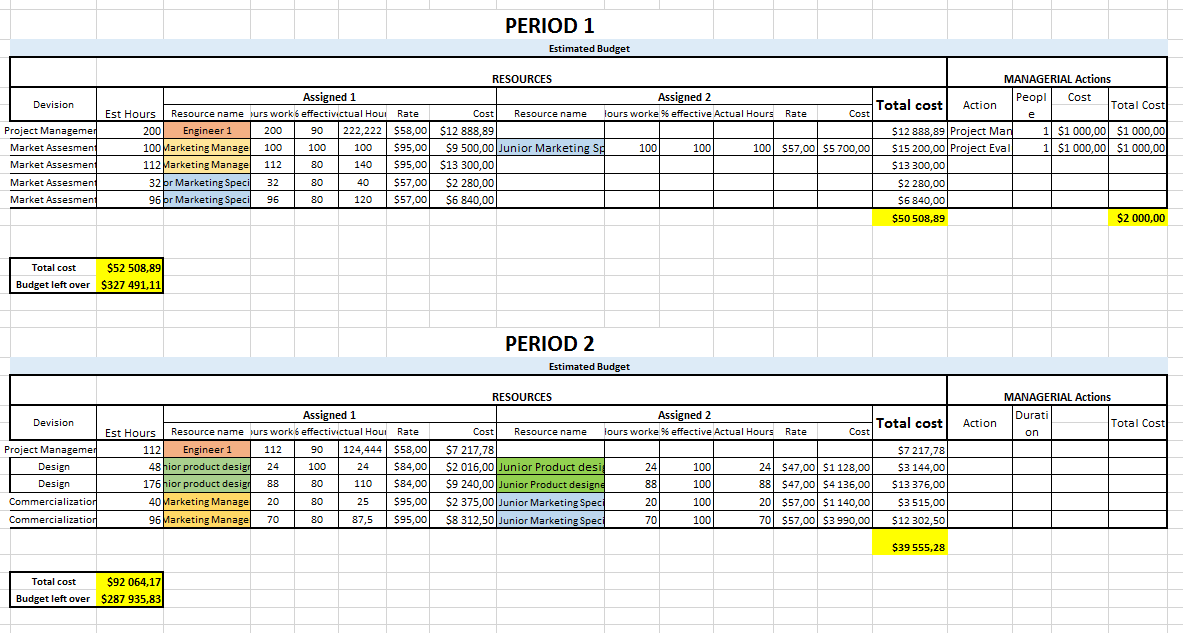
\includegraphics[scale=0.8]{budget_forecast_est_12.PNG}
\caption{Budget Forecast from estimation (period 1 and 2)}
\end{figure}
\begin{figure}[H]
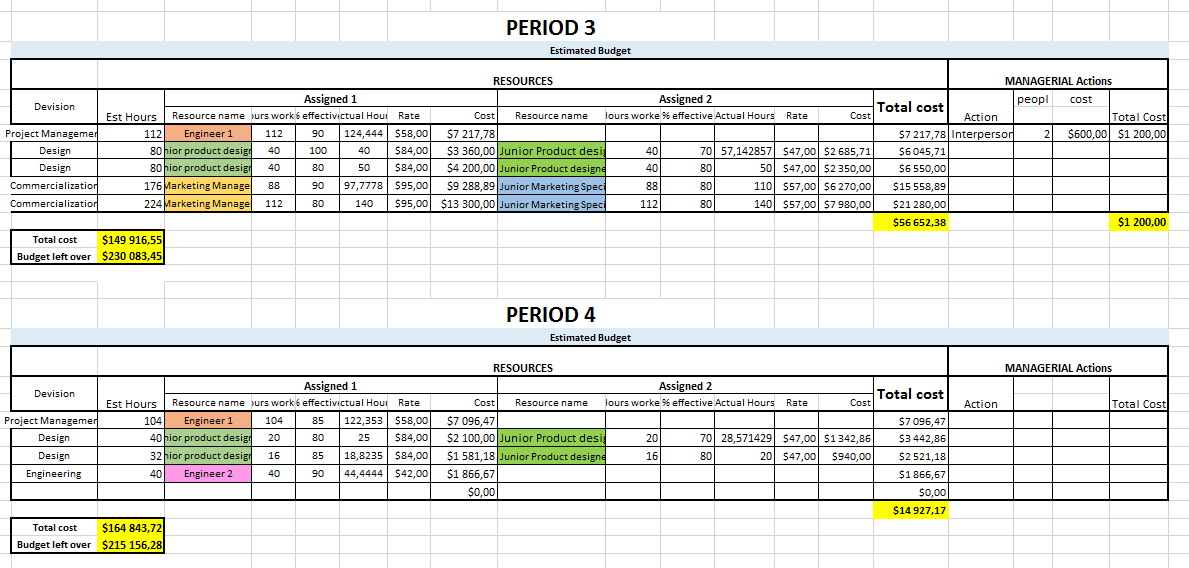
\includegraphics[scale=0.8]{budget_forecast_est_34.PNG}
\caption{Budget Forecast from estimation (period 3 and 4)}
\end{figure}
\begin{figure}[H]
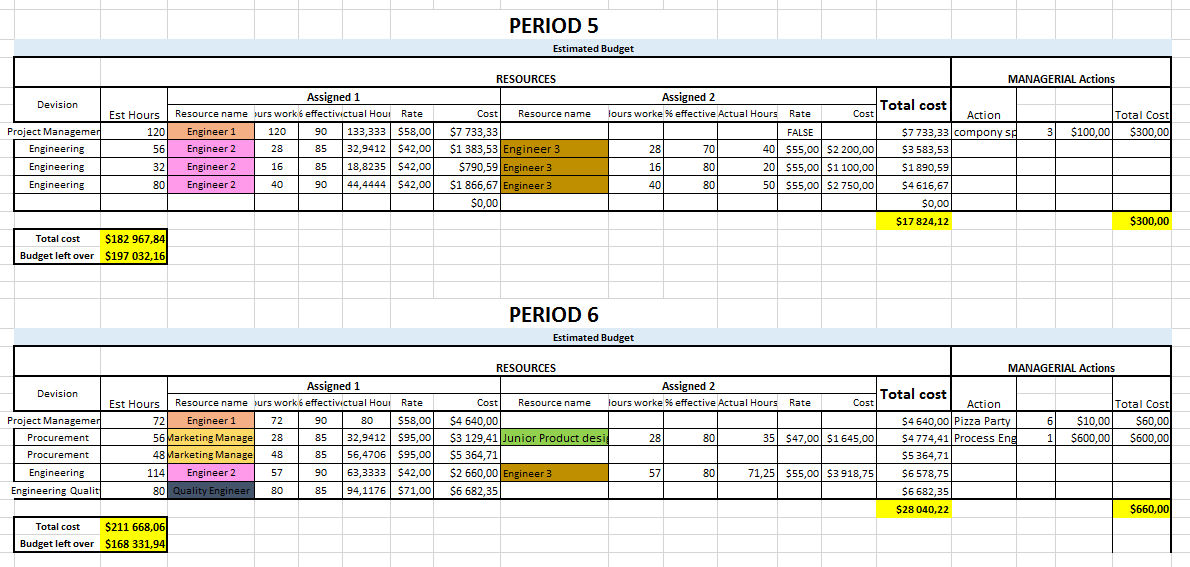
\includegraphics[scale=0.8]{budget_forecast_est_56.PNG}
\caption{Budget Forecast from estimation (period 5 and 6)}
\end{figure}
\begin{figure}[H]
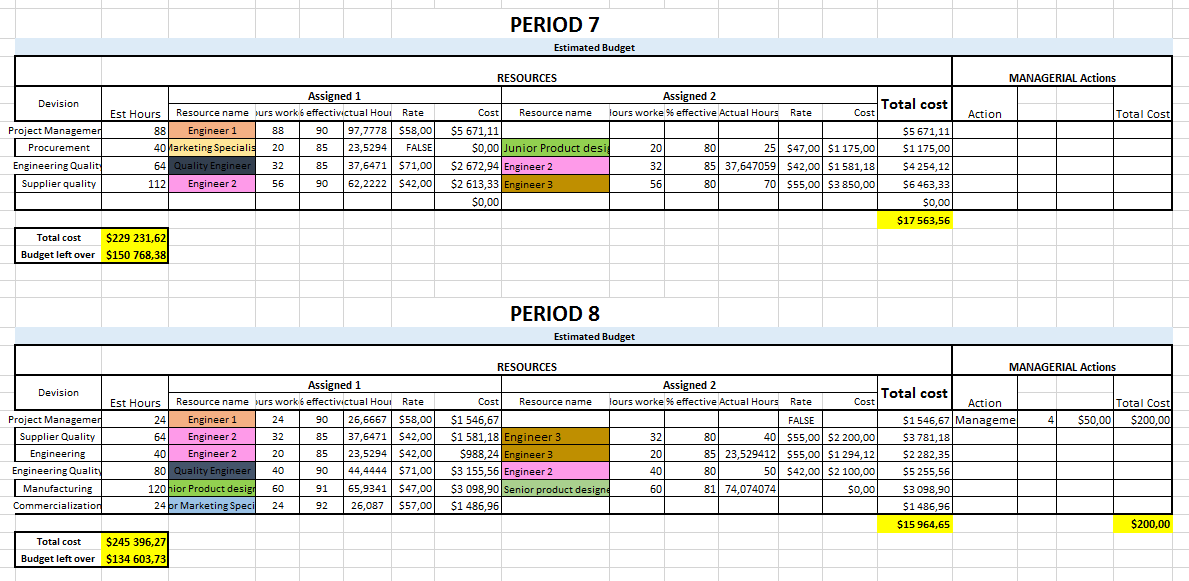
\includegraphics[scale=0.8]{budget_forecast_est_78.PNG}
\caption{Budget Forecast from estimation (period 7 and 8)}
\end{figure}
\begin{figure}[H]
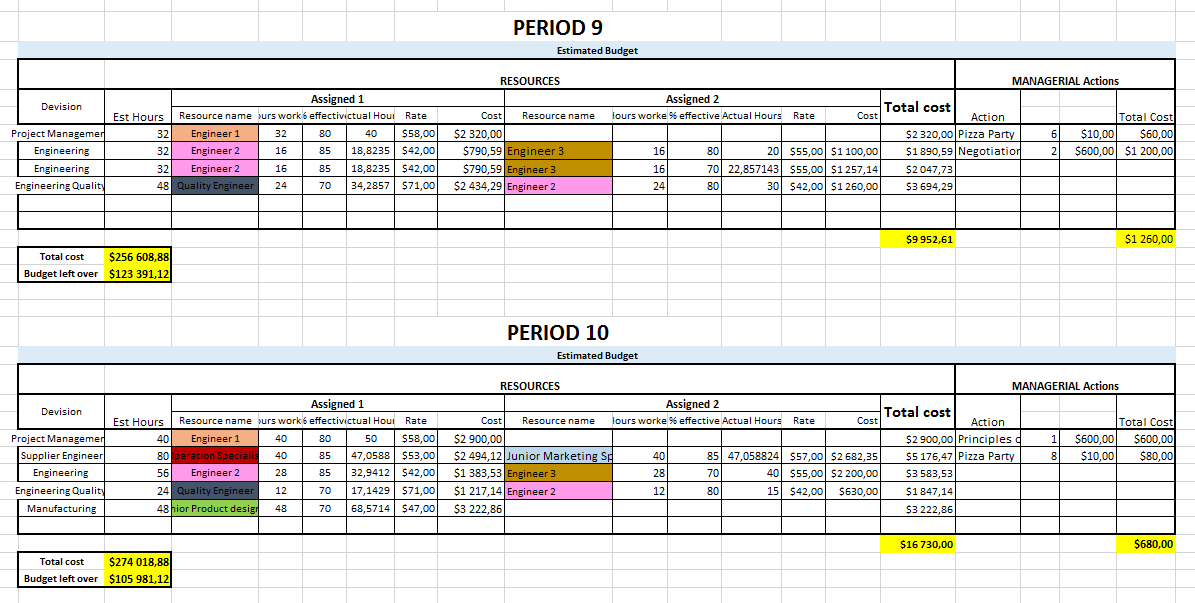
\includegraphics[scale=0.8]{budget_forecast_est_910.PNG}
\caption{Budget Forecast from estimation (period 9 and 10)}
\end{figure}
\begin{figure}[H]
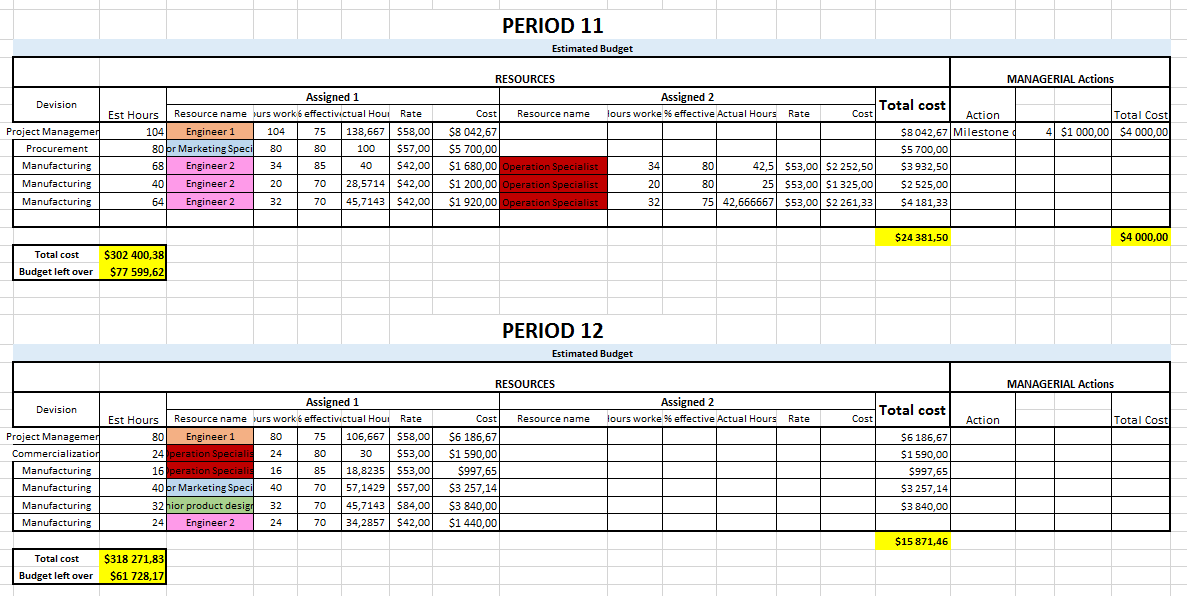
\includegraphics[scale=0.8]{budget_forecast_est_1112.PNG}
\caption{Budget Forecast from estimation (period 11 and 12)}
\end{figure}

\end{landscape}

\section{Risk Register}
\section{Meeting Minutes}

\end{appendices}


% \begin{figure}[H]
% \begin{subfigure}{0.5\textwidth}
% 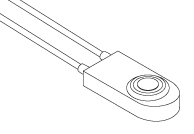
\includegraphics[scale=0.3]{3.png}
% \caption{Pushbutton Switch.\\
% Reproduced from \cite{cpi}.}
% \label{fig:p}
% \end{subfigure}
% \begin{subfigure}{0.5\textwidth}
% \centering
% 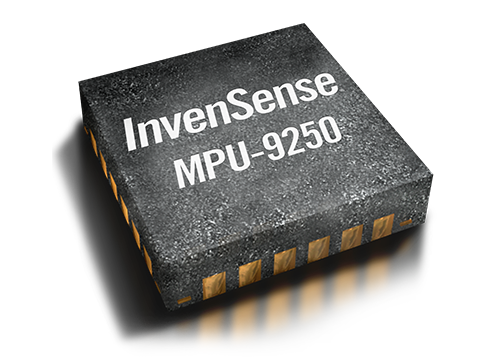
\includegraphics[scale=0.1]{2.png}
% \caption{InvenSense MPU-9250.\\
% Reproduced from\cite{iven}.}
% \label{fig:att}
% \end{subfigure}
% \begin{subfigure}{0.5\textwidth}
% \centering
% 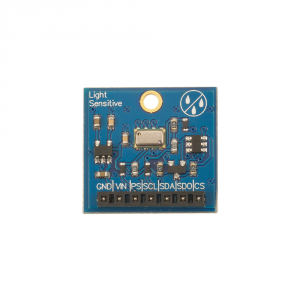
\includegraphics[scale=0.3]{1.png}
% \caption{Altimeter Module MS5607.\\ Reproduced from \cite{par}.}
% \label{fig:pres}
% \end{subfigure}
% \caption{Sensors}
% \label{fig:sensors}
% \end{figure}


% In order for the data to be transmitted successfully, it needs to be in a format acceptable by the GCS. The data will be stored in a JSON packet created using a C++ library\cite{ajson}.

% Code block \ref{code:json1} shows a potential data packet.

% \lstset{language=html,caption={Potential packet},label=code:json1}
% \begin{lstlisting}
% {
%   "temperature": "11.3",
%   "pressure": "99.325"
% }
% \end{lstlisting}

% \begin{figure}
% \centering
% 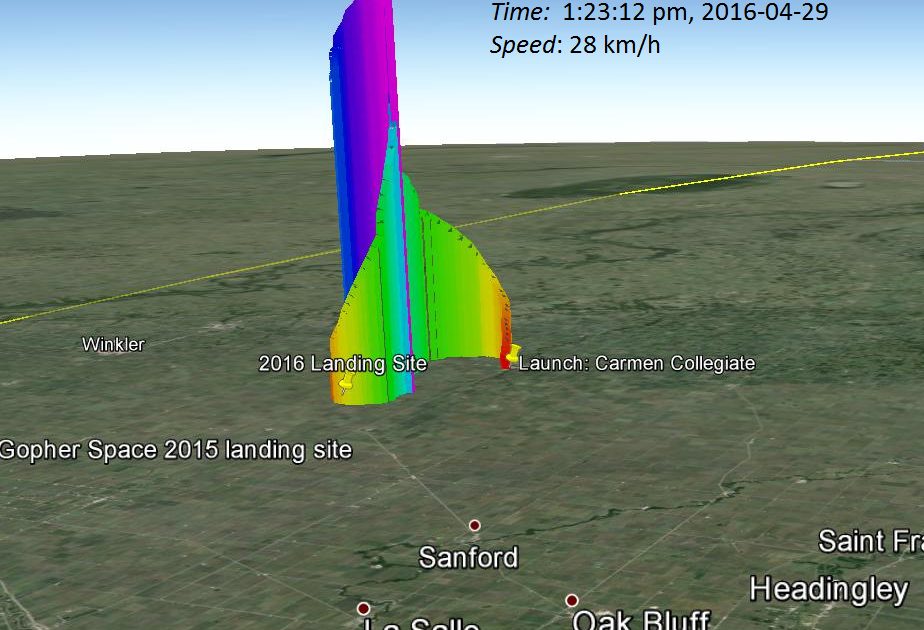
\includegraphics[scale=0.35]{flight_path.png}
% \caption{CanSat flight trajectory\\
% Reproduced from \cite{gopher}}
% \label{fig:flight_path}
% \end{figure}




% \subsection{How to add Tables}

% Use the table and tabular commands for basic tables --- see Table~\ref{tab:widgets}, for example. 

% \begin{table}
% \centering
% \begin{tabular}{l|r}
% Item & Quantity \\\hline
% Widgets & 42 \\
% Gadgets & 13
% \end{tabular}
% \caption{\label{tab:widgets}An example table.}
% \end{table}

% \subsection{How to write Mathematics}

% \LaTeX{} is great at typesetting mathematics. Let $X_1, X_2, \ldots, X_n$ be a sequence of independent and identically distributed random variables with $\text{E}[X_i] = \mu$ and $\text{Var}[X_i] = \sigma^2 < \infty$, and let
% \[S_n = \frac{X_1 + X_2 + \cdots + X_n}{n}
%       = \frac{1}{n}\sum_{i}^{n} X_i\]
% denote their mean. Then as $n$ approaches infinity, the random variables $\sqrt{n}(S_n - \mu)$ converge in distribution to a normal $\mathcal{N}(0, \sigma^2)$.


% \subsection{How to create Sections and Subsections}

% Use section and subsections to organize your document. Simply use the section and subsection buttons in the toolbar to create them, and we'll handle all the formatting and numbering automatically.

% \subsection{How to add Lists}

% You can make lists with automatic numbering \dots

% \begin{enumerate}
% \item Like this,
% \item and like this.
% \end{enumerate}
% \dots or bullet points \dots
% \begin{itemize}
% \item Like this,
% \item and like this.
% \end{itemize}

% \subsection{How to add Citations and a References List}

% You can upload a \verb|.bib| file containing your BibTeX entries, created with JabRef; or import your \href{https://www.overleaf.com/blog/184}{Mendeley}, CiteULike or Zotero library as a \verb|.bib| file. You can then cite entries from it, like this: \cite{greenwade93}. Just remember to specify a bibliography style, as well as the filename of the \verb|.bib|.

% You can find a \href{https://www.overleaf.com/help/97-how-to-include-a-bibliography-using-bibtex}{video tutorial here} to learn more about BibTeX.

% We hope you find Overleaf useful, and please let us know if you have any feedback using the help menu above --- or use the contact form at \url{https://www.overleaf.com/contact}!

\newpage
\bibliographystyle{plain}
% \bibliographystyle{alpha}
\bibliography{references}

\end{document}